\chapter{Dalsza ścieżka rozwoju projektu}
\label{cha:dalsze}

\section{Wprowadzenie zautomatyzowanego systemu testowania projektu}
\section{Migracja do nowego standardu języka C++}
\section{Automatyzacja procesu publikowania produktu}


\chapter{Podsumowanie oraz wnioski}
\label{cha:summary}

\section{Statystyki projektu}
\label{sec:stat}

\appendix
\chapter{Dodatki/Appendixes}
\label{cha:app}

\section{Porównanie początkowej i obecnej struktury projektu oraz kodu źródłowego}
\section{Adding new modules to the project using existing CMake templates}
\label{appendix:A2}

\newpage

\includepdfset{pages=-,pagecommand=\thispagestyle{fancy}}
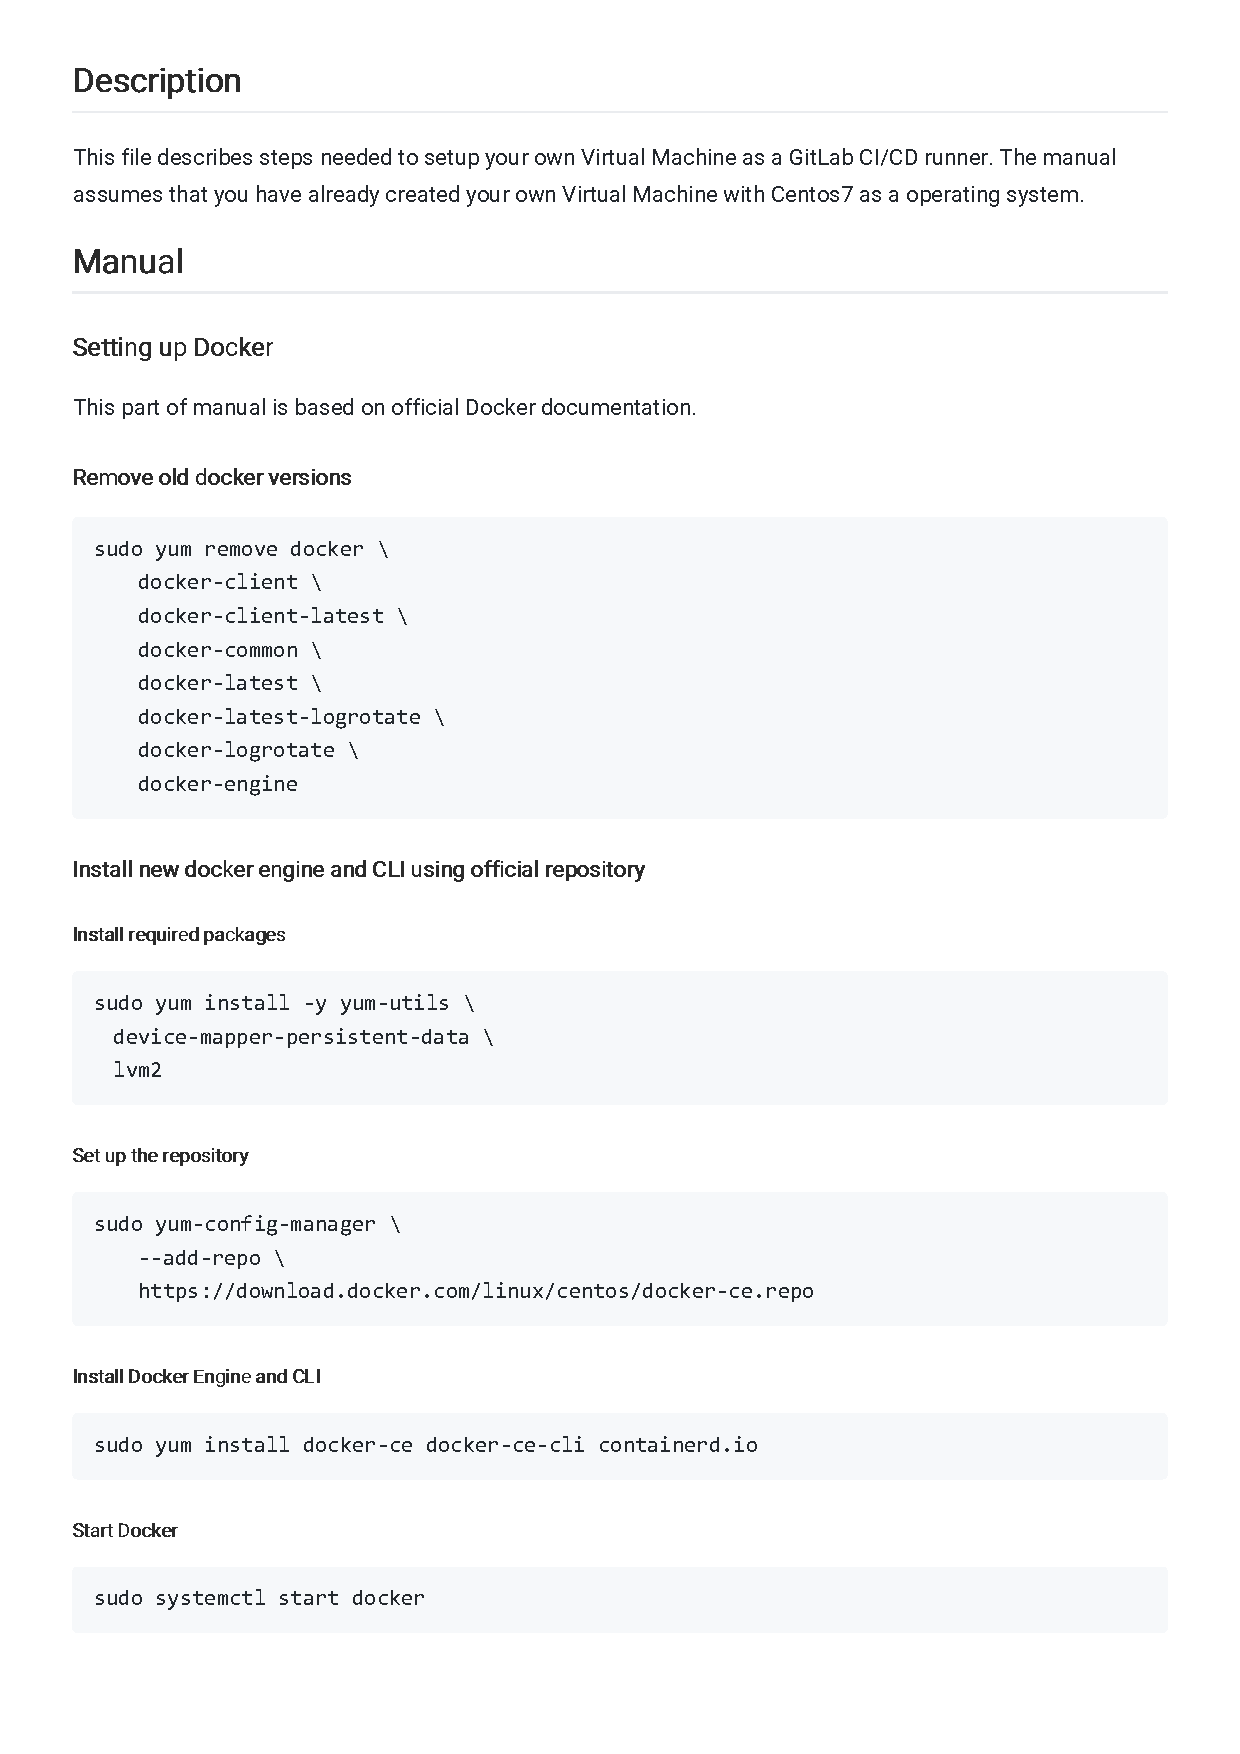
\includepdf[pages=1, scale=0.85,offset= 0.65cm -1cm, pagecommand={\section{Preparing virtual machine to work as a runner\label{appendix:A3}}}]{res/howToRunner.pdf}
\includepdf[pages=2,scale=0.85,offset= 0.65cm 0]{res/howToRunner.pdf}
\includepdf[pages=3,scale=0.85,offset= 0.65cm 0]{res/howToRunner.pdf}

Dodatek \ref{appendix:A3} opisuje procedurę dodawania nowej maszyny jako \textbf{GitLab CI/CD Runner}, czyli jednostka odpowiedzialna za wykonywanie zadań w ramach funkcjonalności \textbf{GitLab CI/CD}. Instrukcja zakłada, że maszyna posiada zainstalowany system operacyjny \textbf{Linux} w dystrybucji \textbf{Centos7}. Wynikem wykonanie wszystkich czynności powinno być dodanie maszyny do panelu \textbf{CI/CD>Runners} dla wybranej grupy, co ukazuje Rysunek \ref{fig:runner}. Instrukcja została napisana w oparciu o dokumentację \textbf{Docker}TUTAJREF oraz dokumentację \textbf{GitLab}TUTAJREF.

\begin{figure}
\caption{Panel przedstawiający dodane \textbf{GitLab CI/CD Runner} w ramach projektu.}
\label{fig:runner}
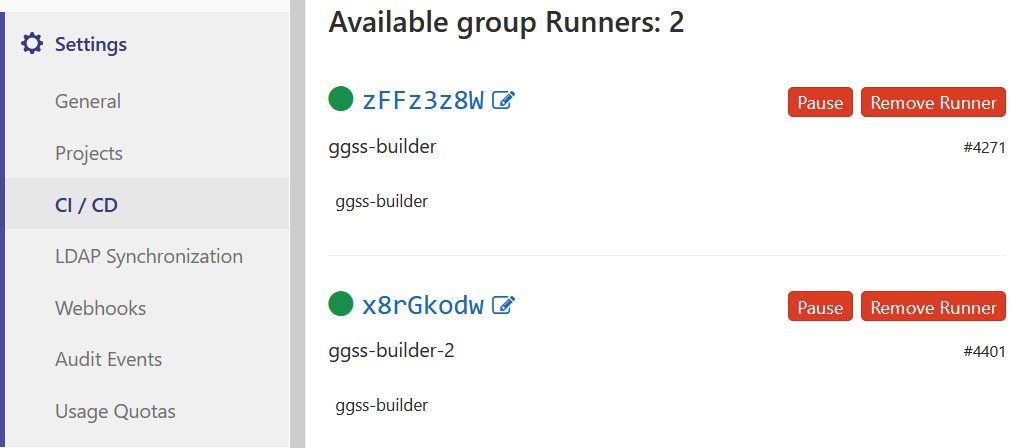
\includegraphics[width=\textwidth]{res/png/runnerAdded}
\end{figure}